\documentclass{beamer}
\beamertemplatenavigationsymbolsempty
\usepackage{amsmath, amssymb, hyperref, graphics}
\usepackage{tikz}

\title{Graph Theory Lecture 15}

\begin{document}
\begin{frame}{What we did last time, what we still have to do}
Last time we stated:
   \begin{theorem}[Euler's formula for graphs on the sphere]
    Let $G$ be a \alert{connected} graph drawn on the sphere without edges crossing.  Let $V$ and $E$ be the number of edges and vertices of $G$, respectively, and let $F$ be the number of faces of the drawing.  Then
    $$V-E+F=2$$
    \end{theorem}
   And explained how together with vertex-edge and face-edge handshaking can be used to prove:
   \begin{itemize}
   \item Every football has 12 pentagons
   \item $K_5$ isn't planar
   \end{itemize}
Today we'll prove Euler's formula, and illustrate more applications.
   \end{frame}

\begin{frame}{Proof(s) of Euler's Theorem }
\begin{block}{Basic proof idea: induction}
  What happens if we delete an edge?

  \begin{itemize}
  \item Number of edges goes down by 1
  \item Number of faces goes down by 1?
  \end{itemize}

  Hence, $V-E+F$ remains unchanged.
\end{block}

\begin{block}{Why the question mark?}
\end{block}
  \end{frame}

\begin{frame}{First(?) proof of Euler's Theorem}
  We induct on the number of faces.

  \begin{block}{Base case: $G$ has only one face}
    \begin{itemize}
    \item Then $G$ has no cycles (Jordan curve theorem)
    \item Assumed $G$ connected, so it's a tree
    \item Therefore $E=V-1$
    \end{itemize}
    \end{block}

  \begin{block}{Inductive step:}
    Assume $G$ has $F>1$ and theorem is true for all graphs with fewer than $F$ faces.
    \begin{itemize}
    \item Then $G$ has an edge separating two faces (why?)
    \item Deleting such an $e$ doesn't disconnected $G$ (why?)
    \item $G\setminus \{e\}$ has one less face, so theorem holds there
      \end{itemize}
       \end{block}

\end{frame}
  
\begin{frame}{Back to videogames}
  Recall that the standard overhead view of a planet in video game produces not the sphere but the torus.
  \begin{definition} A \emph{video game graph} is a graph drawn on a surface so that
    \begin{itemize}
    \item Every vertex has degree 4
    \item Every face has degree 4
    \end{itemize}
  \end{definition}

  \begin{theorem} A video-game graph can never be the sphere.  In fact, a video-game graph will always be the torus or the Klein bottle.
       \end{theorem}
So the video-game designers didn't ``mess up''.
\end{frame}
\begin{frame}{Proof: collect the standard three ingredients}
  \begin{block}{Ingredient 1: Euler's theorem}
    Suppose that $G$ was a video game graph drawn on the sphere: $$V-E+F=2$$
  \end{block}
  \begin{block}{Ingredient 2: Vertex-edge handshaking}
    Since every vertex has degree 4, we have
    $$2E=4V$$
  \end{block}

  \begin{block}{Ingredient 3: Vertex-face handshaking}
    Since every face has degree 4, we have
    $$2E=4F$$
    \end{block}
Mix well to finish proof...
  
  \end{frame}





\begin{frame}{Duality}
  We noticed:
  \begin{itemize}
    \item The cube has $(V, E, F)=(8,12,6)$
    \item The octahedron has $(V, E, F)=(6,12,8)$
  \end{itemize}

  \begin{definition}Let $G$ be a planar connected graph.  The \emph{dual graph} $G^*$ of $G$ has
    \begin{itemize}
    \item One vertex for each face of $G$, placed in the middle
    \item One edge for each edge of $G$, drawn perpendicular
    \item One face for each vertex of $G$
    \end{itemize}
  \end{definition}
\begin{block}{Explains the pattern we saw in $V, E, F$!}
 Face-edge handshaking for $G$ is vertex-edge handshaking for $G^*$, and vice versa.
  \end{block}
  
  \end{frame}

\begin{frame}{Mathematical culture: points for discussion}

\begin{itemize}
\item Euler's Theorem for \emph{other} surfaces
\item ``Dualizing'' our proof of Euler's Theorem: edge contraction
\item Interlacing tree proof of Euler's Theorem
\item Euler's theorem and curvature
\end{itemize}
\begin{center}
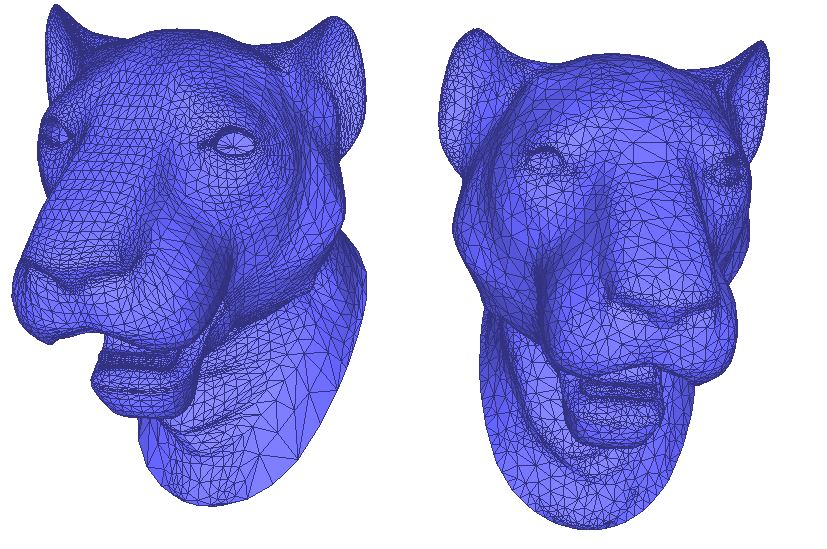
\includegraphics[width=.7\textwidth]{Pictures/mesh.jpg}
\end{center}
\end{frame}


\end{document}
